\documentclass{beamer}

\usepackage{babel}
\usepackage{tikz}
%\usetheme{boxes}
\usepackage[utf8]{inputenc}
\usepackage{amsmath}
\usepackage{amsthm}
\usepackage{hyperref}
\usepackage{natbib}
\usepackage{tikz}
\usepackage{xcolor}
\usepackage[absolute,overlay]{textpos}
\bibliographystyle{plainnat}
\usecolortheme{crane}

\definecolor{orange}{RGB}{232, 86, 15}
\definecolor{blue}{RGB}{14, 159, 232}
\definecolor{blueblue}{RGB}{50, 90, 160}
\definecolor{yellow}{RGB}{232, 187, 14} 
\definecolor{red}{RGB}{232, 14, 59}
\newtheorem{deff}{Definición}
%Information to be included in the title page:
\institute[]{}

\setbeamercolor{title}{bg=blueblue, fg=white}
\setbeamercolor{subttile}{bg=blueblue, fg=white}
\setbeamercolor{frametitle}{bg=blueblue, fg=white}
\setbeamercolor{block title}{bg=blue, fg=white}
\setbeamercolor{block title alerted}{bg=red, fg=white}
\setbeamercolor{block title example}{bg=yellow, fg=white}
\setbeamercolor{footline}{bg=gray, fg=white}
\beamertemplatenavigationsymbolsempty

	
\newcommand{\indep}{\perp \!\!\! \perp}

\newcommand\blfootnote[1]{%
  \begingroup
  \renewcommand\thefootnote{}\footnote{#1}%
  \addtocounter{footnote}{-1}%
  \endgroup
}


\newcommand\overalert[2]{
	 \only<#1>{
\begin{textblock*}{\textwidth}(.35\textwidth,0.25\textheight)
    \begin{beamercolorbox}[wd=.5\textwidth,center,sep=0.3cm]{block title alerted}
	    #2
    \end{beamercolorbox}
\end{textblock*}
}
}

\newcommand\overexample[2]{
	 \only<#1>{
\begin{textblock*}{\textwidth}(.35\textwidth,0.25\textheight)
    \begin{beamercolorbox}[wd=.5\textwidth,center,sep=0.3cm]{block title example}
	    #2
    \end{beamercolorbox}
\end{textblock*}
}
}


\newcommand\overeblock[2]{
	 \only<#1>{
\begin{textblock*}{\textwidth}(.35\textwidth,0.25\textheight)
    \begin{beamercolorbox}[wd=.5\textwidth,center,sep=0.3cm]{block title}
	    #2
    \end{beamercolorbox}
\end{textblock*}
}
}

\title{Causal Inference}
\author{Gherardo Varando}
\date{IPL \\ 16 May 2023}
\begin{document}

\begin{frame}
	\titlepage
\end{frame}

\begin{frame}{Causal Inference}
	\begin{columns}
		\begin{column}{0.5\textwidth}
			\begin{itemize}
				\item<1-> Estimate the strength of the effect of ENSO on vegetation 
					greenness
				\item<2-> How effective are humanitarian actions to fight food insecurity?  
				\item<3-> there is an effect of precipitation in Denmark into precipitation in the Mediterranean region?  
				\item<4-> What is the effect of radiation on NEE/GPP ?  
					 Or the effect of temperature on RECO? 
			\end{itemize}
		\end{column}
		\begin{column}{0.5\textwidth}
			\only<1>{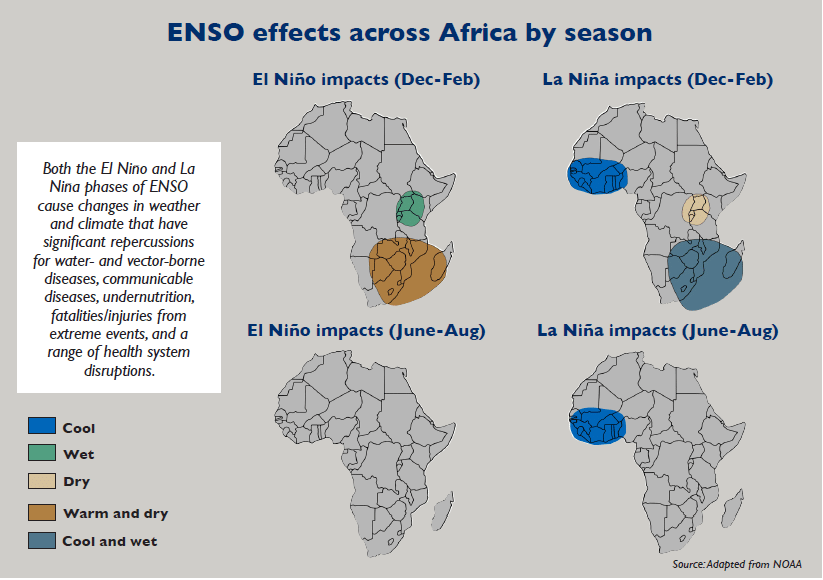
\includegraphics[scale=0.2]{images/Effects-of-ENSO-in-Africa}}
			\only<2>{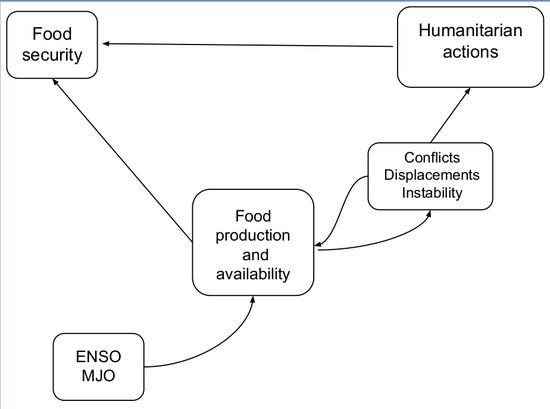
\includegraphics[scale=0.3]{images/foodaction}}
			\only<3>{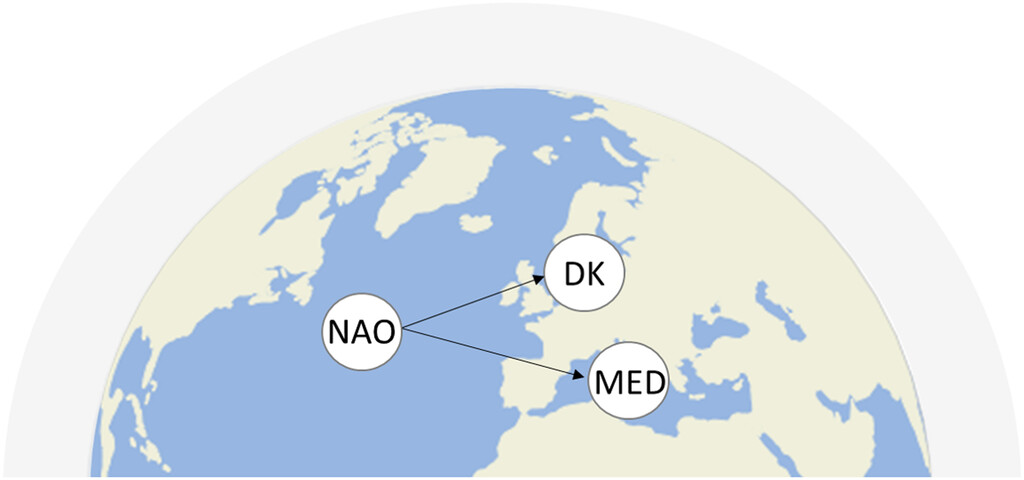
\includegraphics[scale=3]{images/dkmed}}
			\only<4>{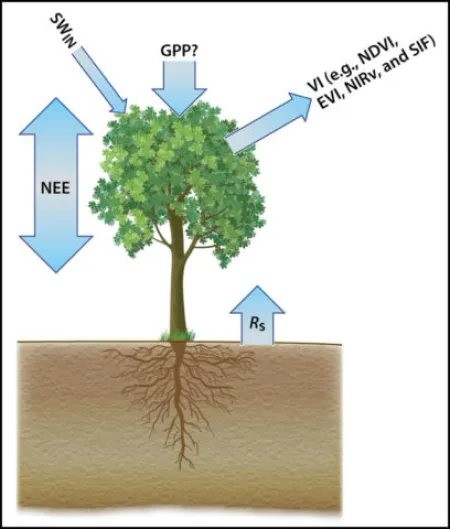
\includegraphics[scale=0.3]{images/nee}}

		\end{column}
	\end{columns}

\end{frame}

\begin{frame}
	\begin{itemize}
		\item Causal link between forest management practices and burned area size, fire severity, post-fire regeneration 
		\item Biomass yield drivers/what if scenarios (management alternatives to optimize productivity)
		\item Applying causal inference methods to study problems that feature social and climate variables
		\item  Estimate the effect of droughts on crop production across Europe  
		\item Estimate the conditional average treatment effect (CATE) of major crop rotations (in Europe) on yield and/or soil organic carbon using Double Machine Learning (DML) 
		\item ...  
	\end{itemize}

\end{frame}

\begin{frame}{Causal Inference}
	\begin{itemize}
		\item  Estimate average treatment effect (ATE) or 
			conditional average treatment effect (CATE) 
		\item<2-> Usually provide confidence intervals and/or test hypothesis 
		\item<3-> Consider possible biases: confounding, selection biases, estimation biases  
		\item<4-> Usually assume total or partial knowledge of the causal graph 
		\item<5-> SCM or potential outcome frameworks  
	\end{itemize}
\end{frame}

\begin{frame}{What we will discuss}
	\begin{enumerate}
		\item Brief and fast summary of Part I from \emph{Causal Inference: What If} 
			book~\citep{whatif}: randomized trials, observational studies and 
			conditions for identification of causal effects, biases 
		\item Connections with SCM, graphical causal models 
		\item adjustment, backdoor criterion, do-calculus, front-door adjustment~\citep{peters2017elements} 
		\item some examples 
	\end{enumerate}
\end{frame}


\begin{frame}{Potential outcomes - Counterfactual model}
	\begin{itemize}
		\item consider a binary \textbf{treatment variable} $A$ 
			(1: forest management practice (thinning, controlled burns,...) , 0: wild/uncontrolled forest)    
		\item and a binary \textbf{outcome} $Y$ (1: burned area, 0: not burned) 
		\item $A,Y$ are random variables that take possible different values for each individual
		\item<2-> denote with $Y^{a=1}$ (Y under treatment $a=1$) the outcome variable that would have been observed under treatment $a=1$, and similarly $Y^{a=0}$ 
		\item<2-> $Y^{a=1}$ and $Y^{a=0}$ are called \textbf{potential outcomes} or \textbf{counterfactual outcomes} 
		\item<3-> for each individual, only one of the potential outcomes 
			is actually observed/factual. 
			\[ Y = Y^{a=A}  \quad \text{(consistency equation)} \]
	\end{itemize}
	\blfootnote{\citet{whatif, wasserman2004all}}

\end{frame}

\begin{frame}{Causal effects}
	\begin{definition}{Average causal effects}
		An average causal effect of treatment $A$ on outcome $Y$ is present if 
		\[ P(Y^{a=1} = 1) \neq   P(Y^{a=0} = 1) \]
		or equivalently (for binary outcomes)
		\[ \mathbb{E}[Y^{a=1}] \neq \mathbb{E}[Y^{a=0}] \]
	\end{definition}
	\begin{itemize}
		\item<2-> in practice we need to \textbf{measure} causal effects 
		\item<3-> {causal risk difference} $P(Y^{a=1} = 1) - P(Y^{a=0} = 1)$
		\item<4-> {causal risk ratio} $\frac{P(Y^{a=1} = 1)}{P(Y^{a=0} = 1)}$ 
		\item<5-> {causal odds ratio} $\frac{P(Y^{a=1} = 1) / P(Y^{a=1} = 0) }{P(Y^{a=0} = 1) / P(Y^{a=0} = 0)}$ 
	\end{itemize}
\end{frame}

\begin{frame}{Randomized experiments}
	\begin{itemize}
		\item<1-> We collect data following a randomized control study: 
			for each individual (forest unit/patch)  we flip a coin and we assign the treatment variable 
			to be $a=1$ if heads and $a=0$ if tails. 
		\item<2-> We then collect the outcome variable $Y$ (e.g. burned or not after 1 year) for all individuals in 
			the study (imagine infinite data or all the population is studied) 
		\item<3-> assume no problem with the study, everybody is following instruction and 
			there are no measurements problems (\emph{ideal randomized experiment})  
		\item<4-> can we say something about the causal effect of $A$ on $Y$ ? 
		\item<5-> yes! we can compute the average causal effect ... formally because there
			is \textbf{exchangeability} between the treated ($A=1$) and untreated ($A=0$) groups  
		\item<6-> formally exchangeability is $Y^a \indep A$ (\textbf{careful, not} $Y \indep A$ !!)  
			\overeblock{7}{
				
\includegraphics[scale=0.5]{images/moneyforest}

				What if we do not have enough money for treating (managing the forest patch) in half of the population? What if we have a limit on the funding available ? can we still perform 
			an (ideal) randomized experiment ? }
	\end{itemize}
\end{frame}

\begin{frame}
	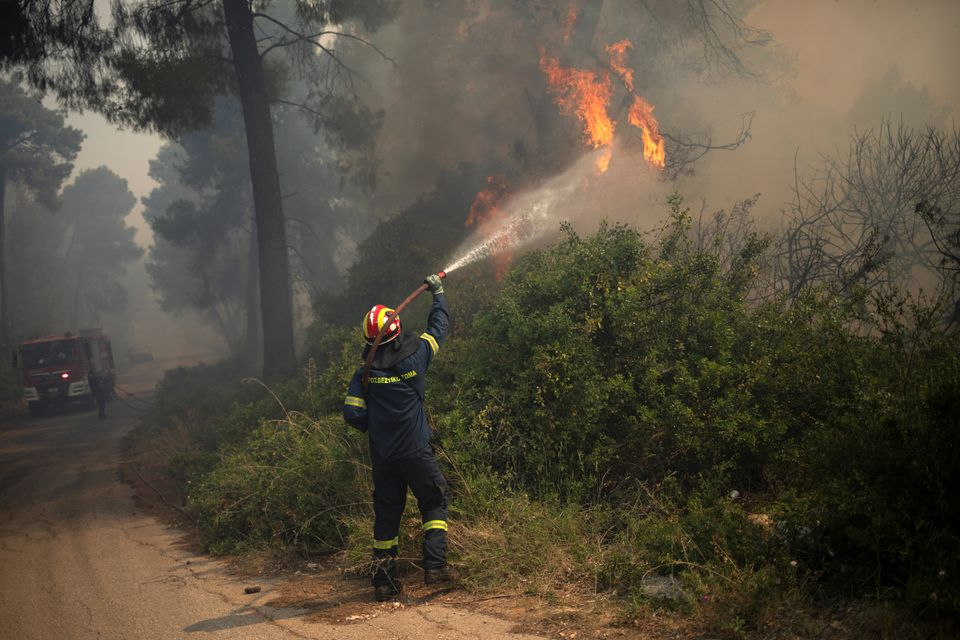
\includegraphics[scale=0.2]{images/fire}

	\textbf{New problem: the firefighters do not like your randomized study} 
	they say that it is too dangerous not to manage some patches at all, and that some 
	areas have a too high fire risk to be left completely untreated 
\end{frame}

\begin{frame}{Conditional randomized experiments}
	\begin{itemize}
		\item<1-> Assume we have now a covariate $L$, measured before treatment was assigned  
			 (e.g. risk of fire: low, medium, high) 
		\item<2-> We divide the population into strata based on the levels of $L$ 
			and we perform randomization with different probabilities in each stratum 
			(e.g. 0.8 for low fire risk, 0.5 for medium fire risk, and 0.2 for high fire risk) 
		\item<3-> In each stratum, we have exchangeability and (if) we are in an 
			ideal randomized study setting thus we can compute 
			average treatment effects 
			(e.g. suppose we obtain risk ratios $P(Y^{a=1} = 1|L)/P(Y^{a=0} = 1|L)$ 
			$0.002/0.001 = 2 $, $0.001 / 0.005 = 0.2 $ and $0.01 / 0.2 = 0.05$) 
		\item<4-> this is called \emph{stratification} and since the causal effect measured are
			different in each stratum we say that there is \emph{effect modification} by $L$ 
		\item<5-> moreover we say that this procedure ensure \textbf{conditional exchangeability}                          $Y^a \indep A | L$ 
	\end{itemize}
\end{frame}

\begin{frame}{Computing ATE from conditionally randomized data} 
	\begin{itemize}
		\item<1-> From the data collected with a conditionally randomized experiment we can compute 
			the ATE in all population. 
		\item<2-> \textbf{Standardization} consists in computing the 
			marginal counterfactual risk 
			as the weighted average of the stratum-specific risk. 
			\[ P(Y^a = 1) = \sum P(Y^a = 1| L = l)P(L = l) \]
		\item<3-> \textbf{Inverse Probability Weighting} is an alternative, but equivalent, 
			procedure to compute $P(Y^a = 1)$ by weighting each individual sample
			by $w_l = 1 / P(A = a|L = l)$ and then we compute $P(Y^a = 1) = \sum w_l P(Y | A= a, L = l)$
	\end{itemize}
	\overeblock{4}{
\small
		remember we obtained risk ratios 

	                 $P(Y^{a=1} = 1|L)/P(Y^{a=0} = 1|L)$ 
			$0.002/0.001 = 2 $, 
			$0.001 / 0.005 = 0.2 $ and 
			$0.01 / 0.2 = 0.05$ in strata with
			treatment probabilities $0.8$, $0.5$ and $0.2$ for low, medium and high 
			risk areas. What is the risk ratio in the entire population ? }
\end{frame}



\begin{frame}{Observational studies}
	Sometimes is unethical, too expensive or simply impossible to conduct experiments, so we are left only with observational data, what can we do? (e.g. we just collect historical 
	data on forest management practice  and burned areas) 
	\begin{itemize}
		\item<2-> Problems: confounding variables (e.g. forest are controlled more when we expect to
			have high risk of fire, patients are treated with more invasive/effective treatments when doctors thinks the case is more serious, \ldots) 
		\item<3->  still under certain conditions and assumptions we can identify the 
			causal effect 
		\item<4-> this conditions \emph{assure that the observational study can be used 
			somehow as a randomized trial} 
	\end{itemize}
\end{frame}

\begin{frame}{Identifiability conditions}
	\begin{enumerate}
		\item<1-> \textbf{Exchangeability} the conditional probability 
			of receiving every value of treatment, though
			not decided by the investigators, depends only on measured covariates $L$
		\item<2-> \textbf{Positivity} the probability of 
			receiving every value of treatment conditional on $L$ is
			greater than zero, i.e., positive
		\item<3-> \textbf{Consistency} the values of treatment under comparison 
			correspond to well-defined interventions that, 
			in turn, correspond to the versions of treatment in the data
	\end{enumerate}
	\only<4>{If we can assume this three conditions we can use the techniques such as IPW or standardization to compute ATE from observational data}
\end{frame}

\begin{frame}{Effect modification}

\begin{itemize}
	\item We say that $V$ is a modifier of the effect of $A$ on $Y$ 
		when the average causal effect of $A$ on $Y$ varies across levels of $V$
	\item \textbf{Stratification} or \textbf{matching} can be used to identify effect modification
	\item<2-> To construct our matched population we replaced the treated in the pop-
ulation by a subset of the treated in which the matching factor $L$ had the
same distribution as that in the untreated.
	\item<3-> they require exchangeability and positivity 
	\item<4-> Standardization (or IPW), stratification and matching measure different 
		causal effects: Average effects in the entire population, conditional causal effects (startification) and usually causal effects in the treated and untreated for matching  
\end{itemize}

\end{frame}

\begin{frame}

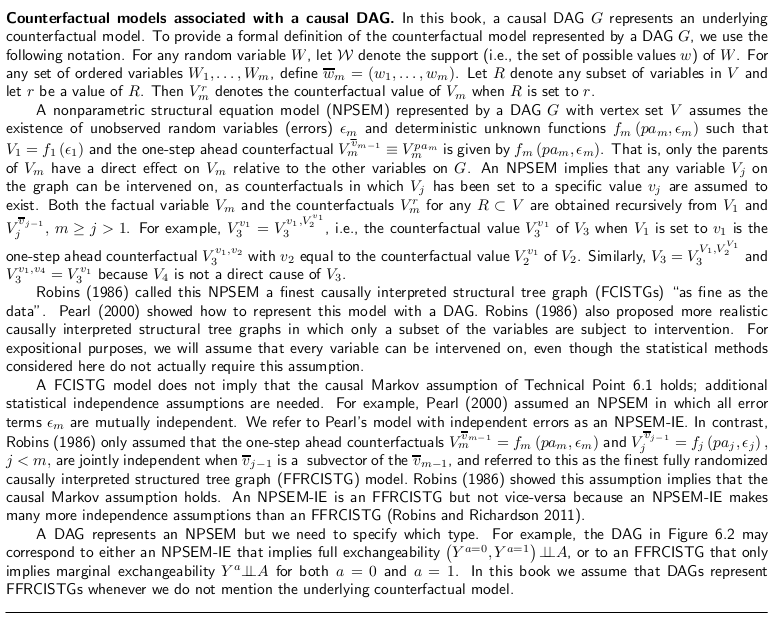
\includegraphics[scale=0.4]{images/dagcon}
\end{frame}

\begin{frame}{Computing interventional distributions in SCM}
	\begin{block}{\small truncated factorization~\citep{pearl1993belief}, 
		G-computation formula~\citep{robins1986new}, 
		manipulation theorem~\citep{spirtes2000causation}}
		Given an SCM $\mathcal{C}$ and an intervened SCM $\tilde{\mathcal{C}}$, obtained 
		from $\mathcal{C}$ by intervening on some $X_k$ with $k \neq j$, we have that 
		\[P^{\tilde{\mathcal{C}}}(X_j |  X_{pa(j)}) = P^{\mathcal{C}}(X_j | X_{pa(j)})\]

	\end{block}
	\begin{itemize}
		\item<1-> Combining the above property and the assumption of SCM we can sometimes
			compute interventional distribution from observational quantities 
		\item<2-> Thus in practical terms we will be able sometimes to 
			estimate interventional objects, such as treatment effects, from 
			observational data alone
		\item<3-> This requires the \emph{knowledge of the causal graph} 
	\end{itemize}

	\blfootnote{\citet{peters2017elements}}
\end{frame}

\begin{frame}{Confounding and adjusting}
         \begin{itemize}
		 \item<1-> Consider an SCM $\mathcal{C}$, the causal effect from $X$ to $Y$ is called confounded if $P^{\mathcal{C}, do(X = x)}(y) \neq P^{\mathcal{C}}(y)$ 
		 \item<2-> $\mathbf{Z}$ is called a valid adjustment set for $X,Y$ if 
			 \[ P^{\mathcal{C}, do(X = x)}(y) = \sum P^{\mathcal{C}}(Y| X, \mathbf{Z} = z)P^{\mathcal{C}}(\mathbf{Z}=\mathbf{z}) \]
		 \item<3-> Valid asjustment sets are: 
			 \begin{enumerate}
				 \item \textbf{parent adjustment} $PA_X$ 
				 \item \textbf{backdoor criterion} Any $\mathbf{Z}$ such that i) contains no descendant of X and ii) blocks all backdoor paths $\rightarrow X$ 
				 \item \textbf{towards necessity}  \ldots 
			 \end{enumerate}
		 \item<4-> Valid adjustment sets ensure conditional exchangeability, thus we can use standardization or stratification to compute average or conditional causal effect 
		 \item<5-> viceversa there are techniques that can handle confounding problems without relying on exchangeability: e.g. difference-in-differences, instrumental variables and 
			 the front door criterion
	 \end{itemize}
	\blfootnote{\citet{peters2017elements}}
\end{frame}

\begin{frame}{Selection bias} 
	\begin{center}
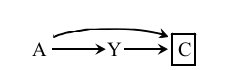
\includegraphics[scale=1]{images/selection}
	\end{center}
	\begin{itemize}
		\item<1-> If we condition on $C$ there are two open paths between $A$ and $Y$ 
		\item<2-> This can happen for example: differential loss to follow-up, missing data bias, nonresponse bias, healthy worker bias, self-selection bias, volunteer bias, 
			and selection affected by treatment received before study entry 
		\item<3-> Selection bias leads to a lack of exchangeability
		\item<4-> IPW or stratification can be used to control for selection bias 
		\item<5-> randomization does not protect from selection bias 
	\end{itemize}
\end{frame}


\begin{frame}{Do-calculus}
	\begin{itemize}
		\item<1-> an interventional distribtuion in an SCM is called identifiable if it can be computed from observational quantities and properties of the graph structure 
		\item<2-> Pearl has developed the so-called \textbf{do-calculus} that consists in a set of three rules: Insertion/deletion of observations, Action/observation exchange, Insertion/deletion of actions
		\item<3-> do-caluclus is complete, every identifiable interventional distribution can be obtained 
		\item<4-> one corollary of the do-calculus theorem is the \textbf{front-door adjustment} 
	\end{itemize}

\end{frame}

\begin{frame}
	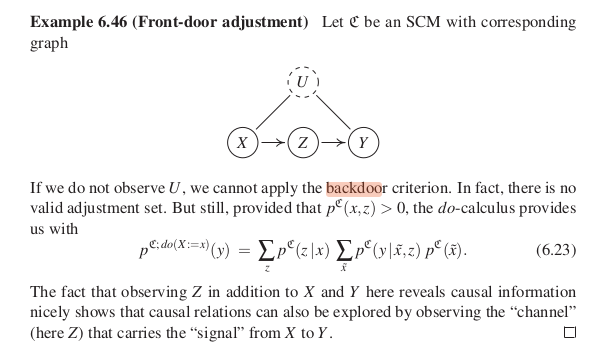
\includegraphics[scale=0.5]{images/front}
\end{frame}

\begin{frame}[allowframebreaks]
\bibliography{biblio}
\end{frame}

\end{document}


